\providecommand{\main}{..}
\documentclass[../COS3712_Notes.tex]{subfiles}

\begin{document}
  \setcounter{chapter}{4}
  \chapter{Viewing}
    \section{Classical and Computer Viewing}
      Projectors meet at the \concept{centre~of~projection~(COP)}.
      The COP corresponds to the centre of the lens in the camera or in the eye,
      and in a computer graphics system, it is the origin of the \concept{camera~frame}
      for perspective views.
      The projection surface is a plane, and the projectors are straight lines.

      Both classical and computer viewing allow the viewer to be an infinite distance
      from the objects.
      As we move the COP to infinity, the projectors become parallel, and the COP can be
      replaced by a \concept{direction~of~projection~(DOP)}.
      Also, as the COP moves to infinity, we can leave the projection plane fixed
      and the size of the image remains about the same, even though the COP is infinitely
      far from the objects.
      Views with a finite COP are called \concept{perspective~views};
      views with a COP at infinity are called \concept{parallel~views}.
      For parallel views, the origin of the camera frame usually lies in the projection plane.

      The class of projections produced by parallel and perspective viewing is known as
      \concept{planar~geometric~projections}, because the projection surface is a plane,
      and the projections are lines.
      Both perspective and parallel projections preserve lines;
      they do not, in general, preserve angles.

    \section{Classical Viewing}
      In classical viewing, there is the underlying notion of a \concept{principal~face}.

      \subsection{Parallel Projections}
        \begin{definition}{Orthographic Projections}
          In all orthographic (or orthogonal) views, the projectors are perpendicular
          to the projection plane.
          In a \concept{multiview orthographic projection}, we make multiple projections,
          in each case with the projection plane parallel to one of the principal faces
          of the object.

          The importance of this type of view is that it preserves both distances and angles
          in faces parallel to the view plane,
          and because there is no distortion of either distance or shape in images of these faces,
          multiview orthographic projections are well suited for working drawings.
        \end{definition}

        \begin{definition}{Axonometric Projections}
          If we want to see more faces of our box-like object in a single view,
          we must remove one of our restrictions.

          In \concept{axonometric views}, the projectors are still orthogonal to the
          projection plane, but the projection plane can have any orientation with respect
          to the object.

          If the projection plane is placed symmetrically with respect to the three
          principal faces, we have an \concept{isometric} view.
          If it is placed symmetrically with respect to two, it is a \concept{dimetric} view.
          The general case is a \concept{trimetric} view.

          In an isometric view, a line segment's length in the image space is shorter
          than its length measured in the object space.
          This \concept{foreshortening} of distances is the same in the three principal directions,
          so we can still make distance measurements.
          In the dimetric view, however, there are two different foreshortening ratios;
          in the trimetric view, there are three.
        \end{definition}

        \begin{definition}{Oblique Projections}
          The \concept{oblique} views are the most general parallel views.
          We obtain an oblique projection by allowing the projectors to make
          an arbitrary angle with the projection plane.
          Consequently, angles in planes parallel to the projection plane are preserved.
          These views are the most difficult to construct by hand.
        \end{definition}

      \subsection{Perspective Projections}
        All perspective views are characterised by \concept{diminution} of size.
        When objects are moved farther from the viewer, their images become smaller.
        This size change gives perspective views their natural appearance;
        however, because the amount by which a line is foreshortened depends on how far
        the line is from the viewer, we cannot make measurements from a perspective view.

        The classical perspective views are known as \concept{one-}, \concept{two-} or
        \concept{three-point perspectives}.
        The differences among the cases are based on how many of the three principal directions
        are parallel to the projection plane.
        The one-, two-, and three- prefixed refer to the number of \concept{vanishing~points}:
        points at which lines of perspective meet.

    \section{Viewing with a Computer}
      In computer graphics, we stress the independence of the object specifications
      and camera parameters.
      Hence, to create one of the classical views, the application program must use information
      about the objects to create and place the proper camera.
      The desired view can be achieved by applying a sequence of transformations on each object
      in the scene.
      Every transformation is equivalent to a change of frames.
      The coordinate types used in the viewing process are object, camera, and clip coordinates.

      Hidden-surface~removal occurs after the fragment shader.
      Although an object might be blocked from the camera by other objects,
      even with hidden-surface~removal enabled, the rasterizer will still generate fragments
      for blocked objects within the clipping volume.

      \begin{sidenote}{Viewing Process Operations}
        There are two operations in the viewing process:
        \begin{enumerate}
          \item Position and orient the camera.
            This operation is the job of the model-view transformation.
            After vertices pass through this transformation, they will be represented
            in eye or camera coordinates.
          \item Applying the projection transformation.
            This step applies the specified projection -- orthographic or perspective --
            to the vertices and puts objects within the specified clipping volume
            into the same clipping cube in clip coordinates.

            One of the functions of either projection will be to allow us to specify a view volume
            in camera coordinates, rather than having to scale our object to fit into the
            default view volume.
        \end{enumerate}
      \end{sidenote}

      The current transformation matrix will be the product of two matrices:
      the \concept{model-view~matrix} and the \concept{projection~matrix}.
      The model-view~matrix will take vertices in object coordinates and convert theme
      to a representation in camera coordinates and thus must encapsulate the positioning
      and orientation of the camera.
      The projection matrix will both carry out the desired projection,
      and convert a viewing volume specified in camera coordinates to fit inside the viewing
      cube in clip coordinates.

      \begin{figure}
        \begin{center}
          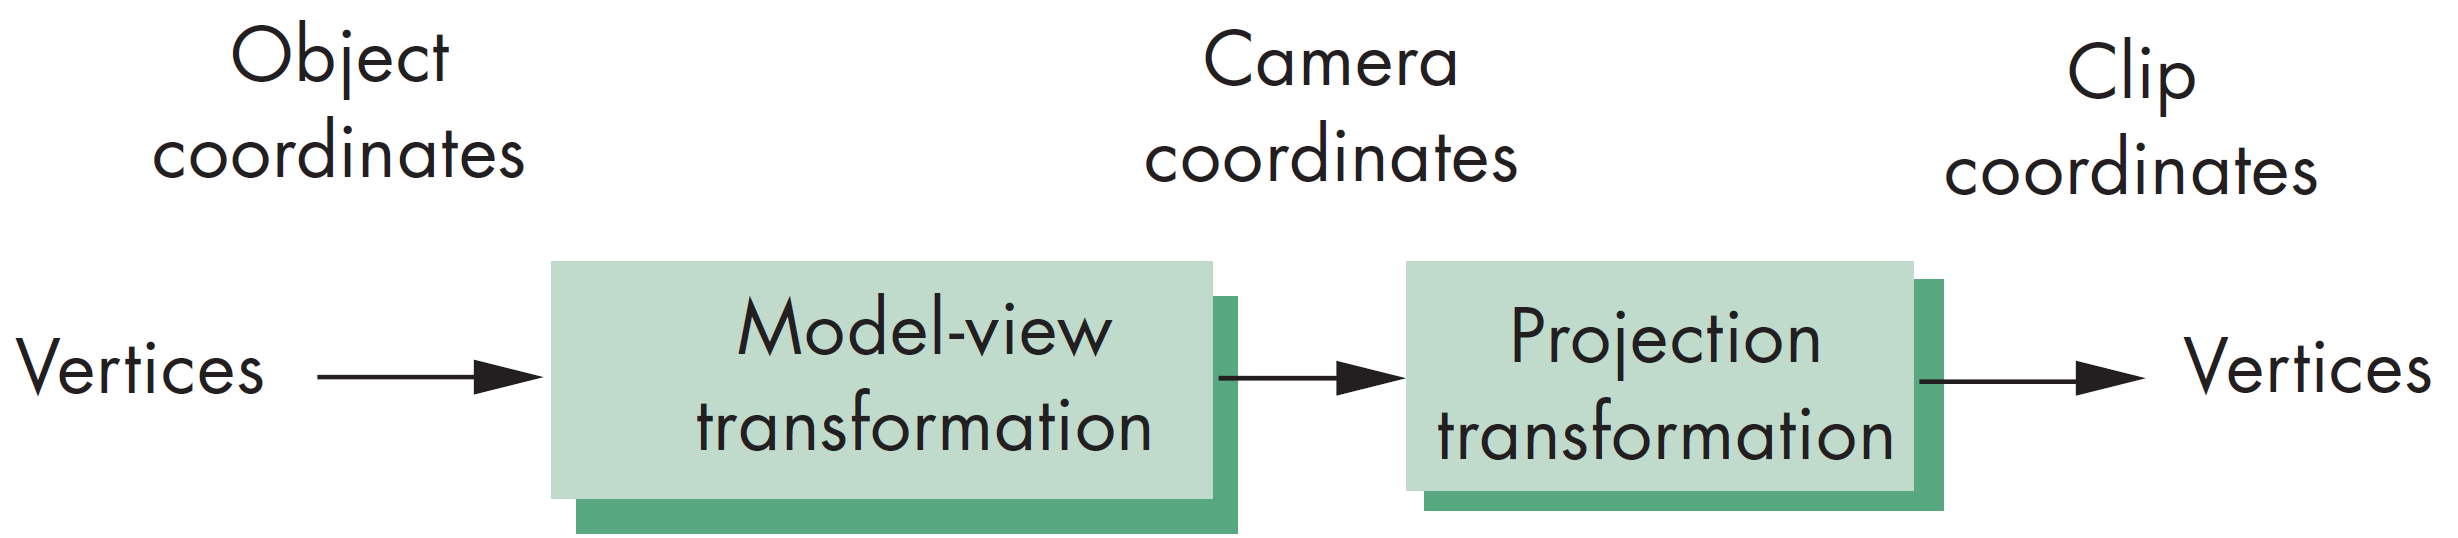
\includegraphics[width=0.8\textwidth]{\main/images/chapter05/viewing_transformations.png}
        \end{center}
        \caption{Viewing Transformations}
      \end{figure}

\end{document}
